        % Research paper grounded in the completed four-policy benchmark exports.
        % Compile from the repository root with IEEEtran.
        \documentclass[conference]{IEEEtran}
        \usepackage{graphicx,booktabs,amsmath,amssymb,url}
        \usepackage{cite}
        \graphicspath{{research/results/final/graphs/}}
        \setlength{\emergencystretch}{2em}

        \begin{document}
        \title{A Containerized Testbed for Latency-Aware Task Offloading Between Edge and Cloud Workers}
        \author{\IEEEauthorblockN{Thatha Surya -- AP23110010323, Pitchuka Himasree -- AP23110010267, Uzair N. Syed -- AP23110010307}
        \IEEEauthorblockA{Department of Computer Science and Engineering\\SRM University-AP, Andhra Pradesh, India\\Email: surya\_thatha@srmap.edu.in, himasree\_pitchuka@srmap.edu.in, uzairn\_syed@srmap.edu.in}}
        \maketitle

        \begin{abstract}
        This paper documents a reproducible testbed for comparing task-placement policies across containerized edge and cloud workers. The implementation compares Round Robin, Edge-only, Fewest active tasks, and latency-aware scheduling. The latency-aware scheduler filters ineligible workers and minimizes predicted network round-trip time, queueing, and execution time. The seeded trace is replayed across policies and measurements separate predictions, worker timings, and API response time. A fresh run covered 12 configurations, 50 tasks per policy and repetition, and 30 repetitions: 72,000 measured tasks, all successful. Mean API response times were 48.95 ms (Round Robin), 28.40 ms (Edge-only), 49.02 ms (Fewest active tasks), and 30.26 ms (latency-aware). In paired repetition-mean comparisons with matrix-wide Holm correction, latency-aware was significantly faster than Round Robin in 11 of 12 configurations and faster than Fewest active tasks in all 12; it was significantly slower than Edge-only in four configurations. Results are limited to one host and simulated RTT timers; they do not establish performance on distributed infrastructure or real networks.
        \end{abstract}

        \begin{IEEEkeywords}
        Edge computing, task offloading, latency-aware scheduling, containerized testbed, benchmarking
        \end{IEEEkeywords}

        \section{Introduction}
        Edge computing places computation near data sources, while cloud resources can offer greater configured capacity at the cost of additional network delay. This trade-off motivates task-offloading policies that account for both communication and computation costs \cite{satya,shi,mach}. Yet scheduler output alone is not sufficient to evaluate a system: measured response time also includes queueing, worker execution, API processing, and persistence overhead. Benchmarking methods therefore need a clear description of the workload, system under test, and measurement boundary \cite{varghese}.

        We present a source-audited account of a containerized edge--cloud testbed and analyze the finished experiments retained in the repository. The codebase contains a Node.js API and three persistent worker containers, together with a React frontend, a PostgreSQL store, experiment orchestration, and a Python analysis pipeline. The experiment runner replays seeded task traces through four policies and exports task-level JSON and CSV data. The network profiles in this study are simulated RTT values; workers share the host.

        The paper makes three practical contributions. First, it specifies the implemented scheduling rule and its eligibility constraints. Second, it distinguishes the predictor's estimated latency from simulated network delay, worker queue and execution times, scheduling overhead, and API response time. Third, it reports a new repeated-run comparison of four schedulers across 12 completed 50-task configurations; larger planned workloads are not included.

    \section{Related Work}
    Cloudlets and edge computing motivate placing computation near data sources, while surveys describe the architectures and communication trade-offs that arise when edge and cloud resources are used together \cite{satya,shi,mach,mao_survey,wang_survey}. Offloading research includes joint task assignment and CPU-frequency control, partial computation offloading, and delay-oriented task scheduling \cite{dinh,wang_partial,liu_delay,ren_partial}. Other approaches optimize energy use or coordinate decisions among multiple users, edge servers, and radio resources \cite{you_energy,chen_multi,sardellitti}. These methods solve richer models than the present prototype, which receives independent tasks and does not model radio resource allocation, local-device execution, task dependencies, energy, or partial offloading.

    Several studies formulate offloading as a constrained optimization problem or use stochastic and learning-based policies; their assumptions and objective functions differ from this implementation \cite{zhou_markov,liu_qos,ma_offload}. In particular, Aljobory and Yazici evaluate round-robin processing and compare edge-server selection rules, including the fewest-active-tasks heuristic, in a multi-server MEC model \cite{ma_offload}. We implement this published server-selection heuristic and compare it with Round Robin, Edge-only, and our minimum-predicted-latency rule on the same task traces. This is a method-level baseline comparison, not a reproduction of their mobility, radio, processor-sharing, or full benchmark model.

    Benchmarking research emphasizes that results depend on the workload, system boundary, and measurement method, which should be reported explicitly \cite{varghese}. In that spirit, this study documents the configured worker profiles and trace replay protocol, and separates the scheduler's latency estimate from worker timings and API response time. The experiments characterize this implementation under simulated RTT and same-host execution; they are not a reproduction of the distributed experiments in the cited work.

        \section{Testbed and Scheduling Policies}
        \subsection{System organization}
        The backend contains the HTTP API, experiment runner, scheduler, worker client, and worker service. Three worker processes expose health, metrics, and execution endpoints. The API refreshes worker state, applies a scheduling policy, dispatches a task, and persists outcomes. A separate frontend invokes the API; the Python tools analyze exported results. In the reported experiments, the workers, API, and database run as containers on one host. This setup enables repeatable software experiments but does not model separate host hardware or an actual WAN.

    \begin{figure*}[t]
    \centering
    \includegraphics[width=0.94\textwidth]{research/figures/fig1_architecture.png}
    \caption{Architecture overview supplied with the project. The sketch lists Round Robin, Edge-only, and latency-aware; the completed evaluation also includes the Fewest active tasks baseline. The dashed outline emphasizes the worker containers; the dashboard, API, and PostgreSQL are also Docker Compose services on the same physical host. Capacity and RTT values shown are Compose defaults, and experiment profiles can override them.}
    \label{fig:architecture}
    \end{figure*}

        The workers execute a deterministic integer recurrence for the requested number of iterations and return a checksum. Workload size in million instructions (MI) is used by the scheduler model and queue-work accounting. Iteration count controls the worker's CPU loop; the code does not calibrate iterations against MI. Accordingly, predicted execution time is a model input-derived estimate, not a validated estimate of the worker's measured loop duration.

        \subsection{Eligibility and policy behavior}
        All policies consider worker health, available memory, and minimum capacity constraints. Round Robin scans eligible workers cyclically. Edge-only filters to eligible edge-role workers and selects the first in list order; with the configured list this is edge-1 whenever it is eligible. Fewest-active-tasks selects the eligible worker with the smallest active-task count, with equal-load ties rotated across tied workers in configured list order; this is the server-selection heuristic reported by Aljobory and Yazici, adapted to the available worker metrics \cite{ma_offload}. Latency-aware evaluates eligible nodes and chooses the minimum predicted latency, breaking near-equal ties by node identifier. It rejects invalid or stale network observations rather than treating a missing RTT as zero.

        \subsection{Latency predictor}
        For task workload $W$ (MI), node capacity $C_n$ (MIPS), execution slots $S_n$, work ahead $A_n$ (MI), and configured RTT $D_n$ (ms), the implementation computes
        \begin{align}
        L_n &= D_n + Q_n + E_n, \\
        E_n &= \frac{1000W}{C_n}, \\
        Q_n &= \frac{1000A_n}{C_nS_n}.
        \end{align}
        Here, $A_n$ is the worker-reported sum of active and queued workload. The queue expression assumes an aggregate service rate of $C_nS_n$ and charges the full MI of active work. The network component is one configured RTT for the request--response transaction. The experiment runner passes the profile RTT into the scheduler and simulates it by sleeping for half the configured value before the worker request and half after the response. Probe duration is not used as the scheduler's network estimate.

        \subsection{Recorded timing boundaries}
        The primary outcome in this paper is API response time, measured around the experiment dispatch flow. This is broader than worker service time: it includes API-side work and database operations as well as the simulated delay and worker execution. Worker queue and execution measurements use a monotonic clock at the worker. Scheduling overhead times the scheduler call. Prediction error compares the sum of simulated network delay, worker queue time, and worker execution time with predicted total latency; it excludes API/database overhead. These quantities are not interchangeable.

        \section{Experimental Method}
        \subsection{Completed workload}
        The configured plan defines four workload sizes (50, 100, 250, and 500 tasks), four network profiles, and three capacity profiles. Each of the 12 retained exports uses 50 tasks per policy, 30 repetitions, and one of the four network by three capacity combinations. The same generated trace is replayed across policies within each repetition; policy order rotates by repetition. The completed data therefore contain 12 configurations $\times$ 30 repetitions $\times$ 50 tasks $\times$ 4 policies, or 72,000 task records. All records have succeeded status. Larger task-count configurations are not part of these exports; the configured plan is not evidence that they completed.

        Network profiles configure RTTs in milliseconds as follows: low (5, 10, 25), medium (10, 30, 60), high (20, 50, 100), and asymmetric (5, 40, 15), in edge-1, edge-2, cloud-1 order. Capacity profiles are default, edge-faster, and cloud-faster. The latter two override configured MIPS, slots, and memory values used by the scheduler; these are profile inputs rather than CPU, memory, or parallelism guarantees enforced by the host. All worker containers share the host, so simultaneous load can influence their measured runtime.

        \begin{table}[t]
        \centering\footnotesize
        \caption{Scope of the completed data analyzed in this paper}
        \label{tab:scope}
        \begin{tabular}{@{}lr@{}}
        \toprule
        Item & Completed value \\
        \midrule
        Distinct task-count values & 1 (50) \\
        Network profiles & 4 \\
        Capacity profiles & 3 \\
        Configurations & 12 \\
        Repetitions per configuration & 30 \\
        Tasks per policy and repetition & 50 \\
        Policies & 4 \\
        Task records & 72,000 \\
        Successful task records & 72,000 \\
        \bottomrule
        \end{tabular}
        \end{table}

        \subsection{Analysis and statistical unit}
        The analysis reads only task-level records and uses API response time in milliseconds. Overall means, medians, and nearest-rank 95th percentiles are descriptive summaries across task rows. For policy comparisons, the unit is the repetition: task outcomes within each replay are aggregated to a repetition mean, and paired policies are compared across the 30 repetitions in each configuration. This avoids treating the 1,500 tasks in a configuration as independent experimental repetitions. The reported paired tests are Wilcoxon signed-rank tests on repetition means; Holm correction is applied across all 36 baseline contrasts (three baselines for each of 12 configurations). Statistical significance uses adjusted $p<0.05$.

        \section{Results}
        \subsection{Aggregate response time}
        Table~\ref{tab:overall} summarizes 18,000 task records per policy. Every policy completed all tasks. Edge-only had the lowest pooled mean; latency-aware was 38.2\% faster than Round Robin but 6.5\% slower than Edge-only. The standard deviation is calculated over the 360 per-configuration, per-repetition policy means and is included to describe run-to-run variability. The task-level percentile summaries describe this particular mix of scenarios and should not be interpreted as independent-sample confidence intervals.

        \begin{table}[t]
        \centering\footnotesize
        \caption{API response time over all 12 completed configurations}
        \label{tab:overall}
        \begin{tabular}{@{}lrrrr@{}}
        \toprule
        & Round Robin & Edge-only & Fewest active & Latency-aware \\
        \midrule
        Successful tasks & 18,000 & 18,000 & 18,000 & 18,000 \\
        Mean $\pm$ SD (ms) & 48.95 $\pm$ 17.21 & \textbf{28.40 $\pm$ 11.12} & 49.02 $\pm$ 17.17 & 30.26 $\pm$ 10.66 \\
        Median (ms) & 41.77 & \textbf{24.85} & 41.85 & 27.49 \\
        95th percentile (ms) & 113.73 & \textbf{53.16} & 113.62 & 57.41 \\
        \bottomrule
        \end{tabular}
        \end{table}

        \begin{figure}[t]
        \centering
        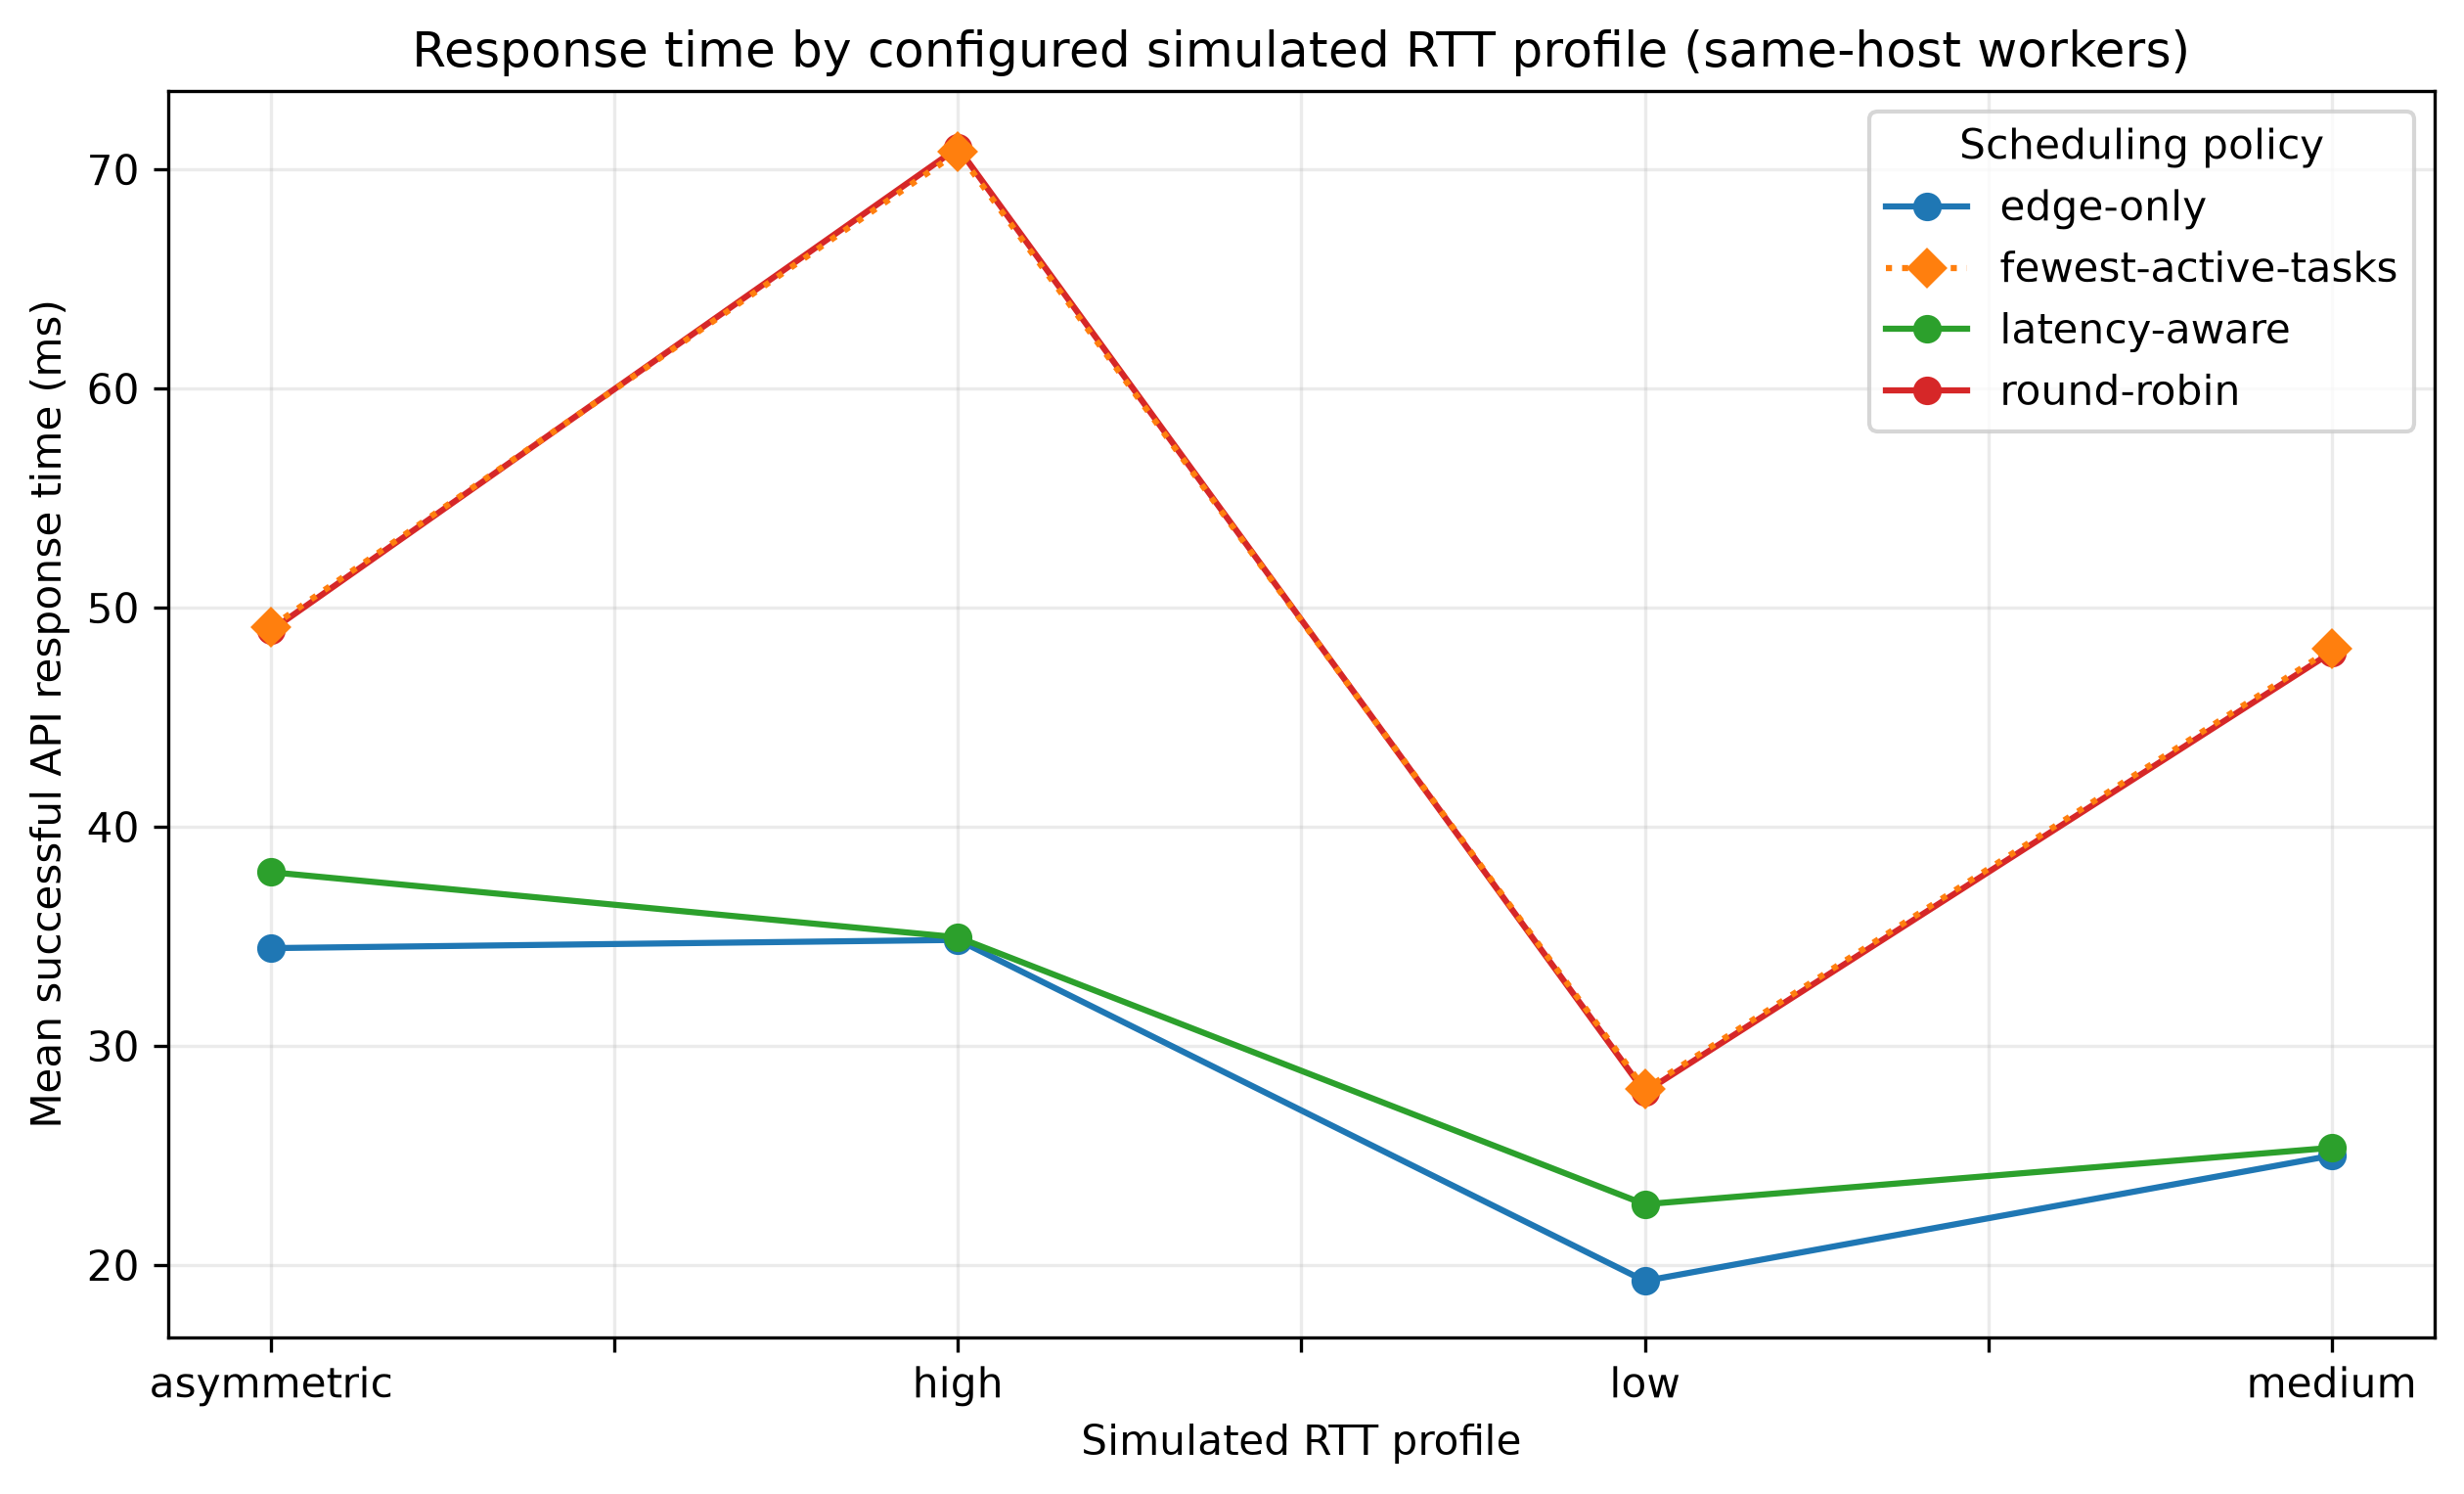
\includegraphics[width=\columnwidth]{research/results/final/graphs/performance_by_rtt.png}
        \caption{Mean API response time by simulated network profile. Each profile mean aggregates the three capacity profiles and 30 repetitions.}
        \label{fig:rtt}
        \end{figure}

        Figure~\ref{fig:rtt} shows the effect of RTT profile on policy response times. Round Robin and Fewest active tasks have similar pooled means, while Edge-only and latency-aware are faster overall. Their relative ordering varies by configuration. As the network profiles are injected timer delays, this result describes policy behavior under controlled synthetic RTT values, not real network performance.

        \subsection{Paired comparisons by configuration}
        Across the 12 configurations, latency-aware has lower repetition-mean response time than Round Robin in all 12; 11 differences remain significant after the global Holm correction. It is faster than Fewest active tasks in all 12 configurations, with all 12 differences significant after correction. The advantage is expected to depend on the configured RTT and capacity trade-off, and should not be generalized beyond the tested inputs.

        For Edge-only, latency-aware has a lower mean in 3 configurations and a higher mean in 9. Four differences favor Edge-only significantly; none favor latency-aware significantly and 8 are not significant. Edge-only places all 18,000 tasks on edge-1; latency-aware places 14,548 on edge-1, 1,169 on edge-2, and 2,283 on cloud-1. Fewest active tasks is faster than latency-aware in all configurations, significantly so after correction. Its placement (6,120 edge-1, 6,119 edge-2, 5,761 cloud-1) closely matches Round Robin, and both have similar pooled response-time means. Evaluating more nodes does not guarantee lower end-to-end API response time because the predictor omits API and database overhead, while its configured MI-to-MIPS estimate is not calibrated to the worker loop.

        \begin{figure}[t]
        \centering
        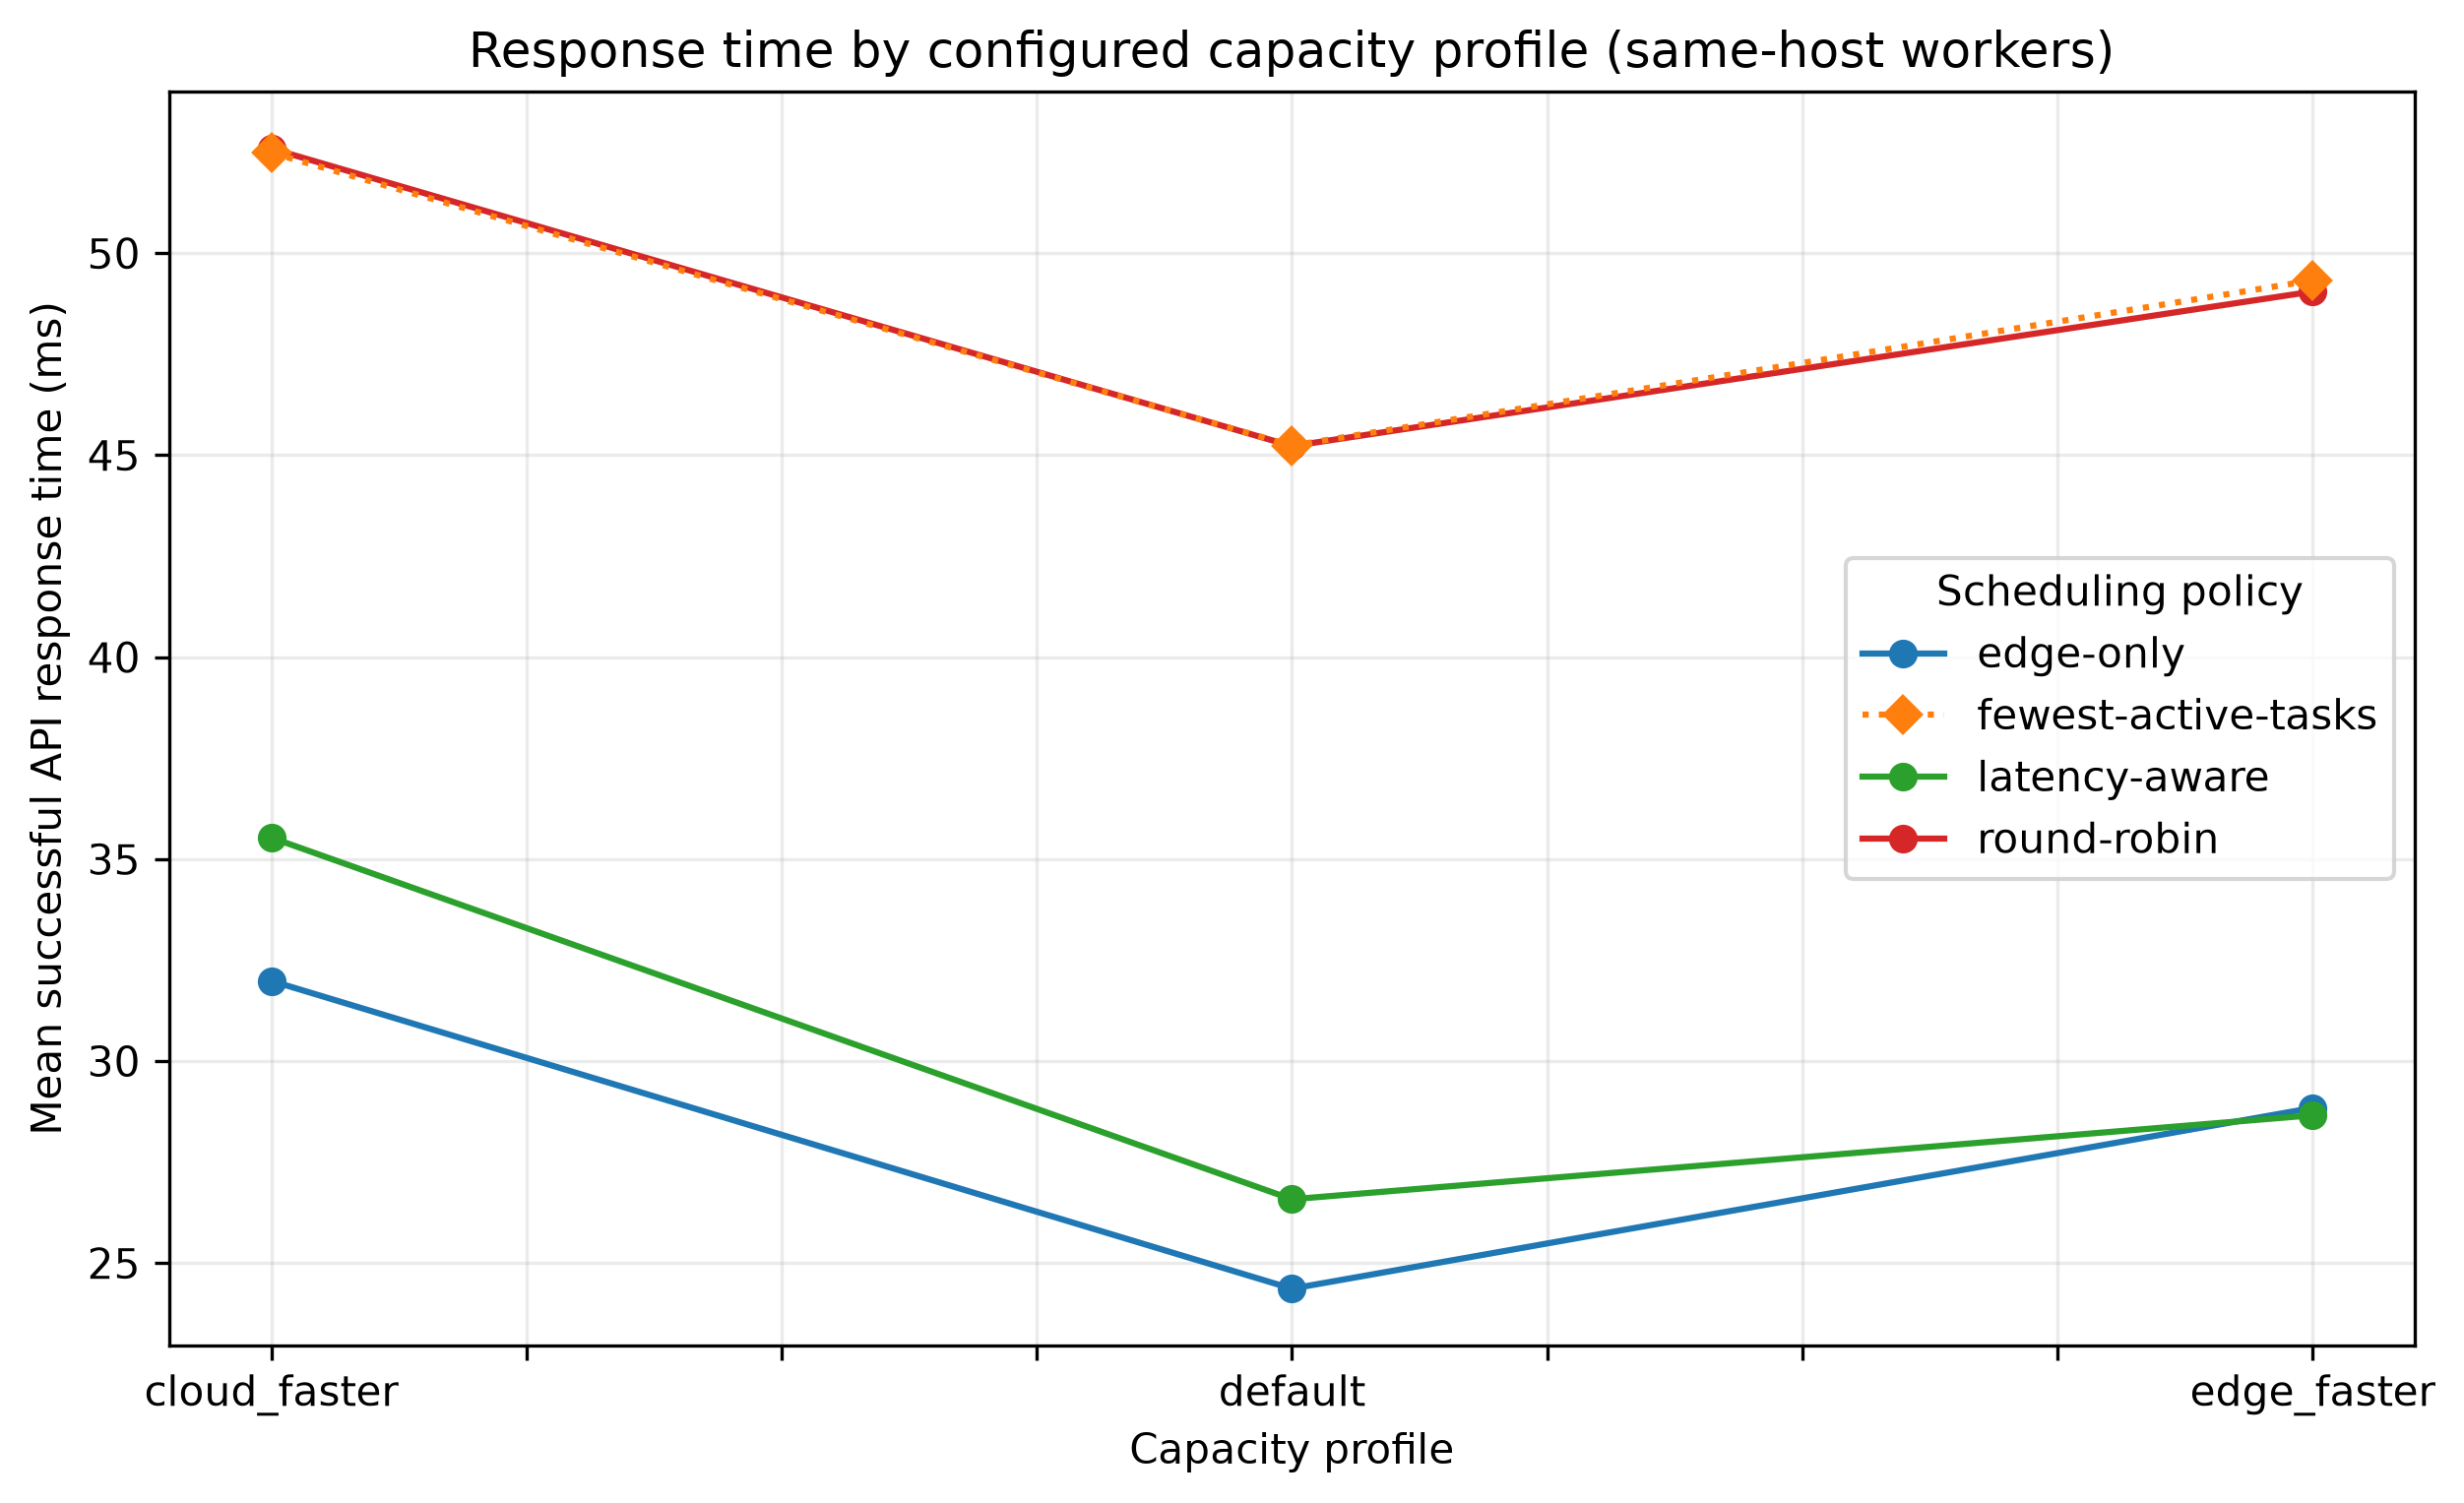
\includegraphics[width=\columnwidth]{research/results/final/graphs/performance_by_capacity.png}
        \caption{Mean API response time by capacity profile. Values aggregate all four simulated network profiles and 30 repetitions.}
        \label{fig:capacity}
        \end{figure}

        The capacity-profile comparison in Fig.~\ref{fig:capacity} illustrates that policy ordering depends on configuration. For example, under the edge-faster profile, means are 49.05 ms (Round Robin), 28.84 ms (Edge-only), 49.33 ms (Fewest active tasks), and 28.66 ms (latency-aware); under cloud-faster they are 52.59, 31.99, 52.49, and 35.53 ms, respectively. These averages are descriptive aggregations and do not replace the paired per-configuration analysis.

        \subsection{Placement and interpretation}
        The observed placement counts help explain the policy differences, but do not demonstrate the predictor's accuracy. Round Robin distributed tasks across all workers (6,120 edge-1, 6,120 edge-2, 5,760 cloud-1). Fewest active tasks had a similar distribution. Edge-only always chose edge-1. Latency-aware used all three nodes with a preference for edge-1. Its mean API response time exceeded Edge-only in the pooled data, which cautions against interpreting minimum predicted latency as minimum measured API response time. The model optimizes a deliberately narrower estimated quantity than the API response outcome analyzed here.

        \section{Limitations and Threats to Validity}
        First, RTT values are static simulated delays applied with timers; there is no packet loss, jitter, congestion, route variation, or physically distant worker. The result therefore says nothing about measured WAN conditions. Second, workers, API, and database share one host. There is no CPU pinning or host isolation, and profile values such as MIPS and slots are scheduler inputs rather than enforced hardware capacities.

        Third, workloadMI is not calibrated against the worker's integer-loop iteration count. Thus, the execution-time estimate may not predict actual worker service time. Fourth, API response time includes API and persistence work that is absent from the predictor, which is a plausible reason that an estimate-minimizing policy does not always minimize the measured API outcome. Fifth, the finished exports cover only taskCount=50. Although the experiment configuration lists 100, 250, and 500, those workloads cannot be analyzed from the available completed raw data. Finally, this benchmark covers four policies but only one worker ordering. Edge-only is a first-eligible-edge baseline, while Fewest active tasks uses instantaneous task counts and rotated tie-breaking; neither models long-term load or resource heterogeneity in the same way as a calibrated scheduler.

        \section{Conclusion}
        We documented the testbed and analyzed 12 completed 50-task configurations, totaling 72,000 successful task records across four policies. Latency-aware was significantly faster than Round Robin in 11 configurations and Fewest active tasks in all 12 after matrix-wide Holm correction. Against Edge-only, it was faster in three and slower in nine, with four significant differences favoring Edge-only; Edge-only had the lowest pooled mean. These findings are bounded by the testbed: network RTT is simulated and workers share a host.

        Further evaluation should complete the larger configured workloads, calibrate workloadMI against worker execution, separate API and persistence timing from task service, add load-aware edge baselines, and use isolated or physically distributed workers with measured or controlled network conditions. Until then, this study is a characterization of the current prototype and its completed benchmark, not evidence of general superiority for latency-aware offloading.

    \section*{Code and Data Availability}
    The project source code, Docker Compose configuration, experiment configuration, completed raw benchmark exports, and analysis scripts are available at \url{https://github.com/uzueer/Edge-Offloading-Research-Application}. The analyzed raw exports, analysis tables, and figures are in \texttt{research/results/final/}. Larger task-count configurations are not included. No archival DOI is cited in this manuscript.

        \begin{thebibliography}{16}
        \bibitem{satya} M. Satyanarayanan, P. Bahl, R. C\'aceres, and N. Davies, ``The case for VM-based cloudlets in mobile computing,'' \emph{IEEE Pervasive Computing}, vol. 8, no. 4, pp. 14--23, 2009, doi: 10.1109/MPRV.2009.82.
    \bibitem{shi} W. Shi, J. Cao, Q. Zhang, Y. Li, and L. Xu, ``Edge computing: Vision and challenges,'' \emph{IEEE Internet of Things Journal}, vol. 3, no. 5, pp. 637--646, 2016, doi: 10.1109/JIOT.2016.2579198.
    \bibitem{mach} P. Mach and Z. Becvar, ``Mobile edge computing: A survey on architecture and computation offloading,'' \emph{IEEE Communications Surveys \& Tutorials}, vol. 19, no. 3, pp. 1628--1656, 2017, doi: 10.1109/COMST.2017.2682318.
    \bibitem{varghese} B. Varghese \emph{et al.}, ``A survey on edge performance benchmarking,'' \emph{ACM Computing Surveys}, vol. 54, no. 3, Art. no. 66, 2021, doi: 10.1145/3444692.
    \bibitem{mao_survey} Y. Mao, C. You, J. Zhang, K. Huang, and K. B. Letaief, ``A survey on mobile edge computing: The communication perspective,'' \emph{IEEE Communications Surveys \& Tutorials}, vol. 19, no. 4, pp. 2322--2358, 2017, doi: 10.1109/COMST.2017.2745201.
    \bibitem{wang_survey} S. Wang, X. Zhang, Y. Zhang, L. Wang, J. Yang, and W. Wang, ``A survey on mobile edge networks: Convergence of computing, caching and communications,'' \emph{IEEE Access}, vol. 5, pp. 6757--6779, 2017, doi: 10.1109/ACCESS.2017.2685434.
    \bibitem{dinh} T. Q. Dinh, J. Tang, Q. D. La, and T. Q. S. Quek, ``Offloading in mobile edge computing: Task allocation and computational frequency scaling,'' \emph{IEEE Transactions on Communications}, vol. 65, no. 8, pp. 3571--3584, 2017, doi: 10.1109/TCOMM.2017.2699660.
    \bibitem{wang_partial} Y. Wang, M. Sheng, X. Wang, L. Wang, and J. Li, ``Mobile-edge computing: Partial computation offloading using dynamic voltage scaling,'' \emph{IEEE Transactions on Communications}, vol. 64, no. 10, pp. 4268--4282, 2016, doi: 10.1109/TCOMM.2016.2599530.
    \bibitem{liu_delay} J. Liu, Y. Mao, J. Zhang, and K. B. Letaief, ``Delay-optimal computation task scheduling for mobile-edge computing systems,'' in \emph{Proc. IEEE ISIT}, 2016, pp. 1451--1455, doi: 10.1109/ISIT.2016.7541539.
    \bibitem{you_energy} C. You, K. Huang, H. Chae, and B. H. Kim, ``Energy-efficient resource allocation for mobile-edge computation offloading,'' \emph{IEEE Transactions on Wireless Communications}, vol. 16, no. 3, pp. 1397--1411, 2017, doi: 10.1109/TWC.2016.2633522.
    \bibitem{chen_multi} X. Chen, L. Jiao, W. Li, and X. Fu, ``Efficient multi-user computation offloading for mobile-edge cloud computing,'' \emph{IEEE/ACM Transactions on Networking}, vol. 24, no. 5, pp. 2795--2808, 2016, doi: 10.1109/TNET.2015.2487344.
    \bibitem{sardellitti} S. Sardellitti, G. Scutari, and S. Barbarossa, ``Joint optimization of radio and computational resources for multicell mobile-edge computing,'' \emph{IEEE Transactions on Signal and Information Processing over Networks}, vol. 1, no. 2, pp. 89--103, 2015, doi: 10.1109/TSIPN.2015.2448520.
    \bibitem{ren_partial} J. Ren, G. Yu, Y. Cai, Y. He, and F. Qu, ``Partial offloading for latency minimization in mobile-edge computing,'' in \emph{Proc. IEEE GLOBECOM}, 2017, doi: 10.1109/GLOCOM.2017.8254550.
    \bibitem{zhou_markov} W. Zhou, W. Fang, Y. Li, B. Yuan, Y. Li, and T. Wang, ``Markov approximation for task offloading and computation scaling in mobile edge computing,'' \emph{Mobile Information Systems}, vol. 2019, Art. no. 8172698, 2019, doi: 10.1155/2019/8172698.
    \bibitem{liu_qos} J. Liu \emph{et al.}, ``QoS driven task offloading with statistical guarantee in mobile edge computing,'' \emph{IEEE Transactions on Mobile Computing}, vol. 21, no. 1, pp. 278--290, 2022, doi: 10.1109/TMC.2020.3004225.
    \bibitem{ma_offload} K. Aljobory and M. A. Yazici, ``Edge server selection with round-robin-based task processing in multiserver mobile edge computing,'' \emph{Sensors}, vol. 25, no. 11, Art. no. 3443, 2025, doi: 10.3390/s25113443.
        \end{thebibliography}

        \end{document}
